\documentclass[a4paper]{article}
\usepackage{amsmath}
\usepackage{amsfonts}
\usepackage{amsthm}
\usepackage{amssymb}
\usepackage[english]{babel}
\usepackage{float}
\usepackage{graphicx}
\usepackage{hyperref}
\usepackage[utf8]{inputenc}
\usepackage{listings}
\usepackage{xcolor}
%% \usepackage{subfigure}
\usepackage{graphicx}
\usepackage{subcaption}
\usepackage{stmaryrd}

\usepackage{a4wide}
\usepackage{url}

\usepackage{appendix}

\graphicspath{{imgs/}} %Setting the graphicspath

\lstset{
  frame=tb,
  language=Python,
  aboveskip=3mm,
  belowskip=3mm,
  showstringspaces=false,
  formfeed=newpage,
  tabsize=4,
  comment=[l]{\#},
  breaklines=true,
  morekeywords={models, lambda, forms}
}

\newcommand{\prob}[1]{\mathbb{P}\left(#1\right)}
\newcommand{\expect}[1]{\mathbb{E}\left(#1\right)}
\newcommand{\bt}[1]{\mathbf{#1}}
\newcommand{\avg}[1]{\sum_{i=1}^{#1}X_i}
\newcommand*{\QEDA}{\hfill\ensuremath{\blacksquare}}%

\newcommand{\nt}{\text}
\newcommand{\lagr}{\mathcal{L}}
\newcommand{\isum}{\sum^\infty_}
\newcommand{\f}{$f$}

\title{\vspace{-5cm} Numerical Optimization \\ Re-exam Handin 4}
\author{Dmitry Serykh (qwl888)}

\begin{document}
\maketitle
\section{The Setup}
I implemented the Trust Region optimizer by following the basic algorithm
structure, outlined Algorithm 4.1. In order to solve the Sub-problem 4.7, I used
the method from Section 4.3, and Algorithm 4.3 in particular, where the root-finding Newton's
Method and Cholesky factorization is used to iteratively find the values of
constant $\lambda$, and consequently the solution to the Sub-problem 4.7 (value
of $p$), such that the conditions from the Theorem 4.1 are satisfied.
\[
\begin{aligned}(B+\lambda I) p &=-g \\ \lambda\left(\Delta-\left\|p\right\|\right) &=0 \\(B+\lambda I) & \text { is positive semi-definite } \end{aligned}
\]

\subsection{Parameters}
I used following parameter values in my implementation. Some values were taken
from the literature, while others were determined empirically.
\begin{itemize}
\item \textbf{Initial trust region radius ($\Delta_0 = 1$)}
\item \textbf{Maximum trust region radius $\tilde{\Delta}=10^3$}
\item \textbf{Lower bound for the actual/predicted reduction ratio $\eta=0.2$}
\item \textbf{Tolerance $\varepsilon = 10^{-7}$ on the gradient magnitude}
\end{itemize}

\section{Testing protocol}
In order to test the effectiveness of my implementation, I came up with a
testing protocol, where I used following metrics:
\begin{itemize}
\item The convergence plots with the number of iteration on the x-scale and the
  Euclidean distance between the current value of $x$ and the
  optimum. The resulting plot can be seen on Figure \ref{plt1}.
\item The convergence plots with the trust region radius.
  The resulting plot can be seen on Figure \ref{plt2}. 
\item \textbf{Accuracy}. The Euclidean distance to the optimum at the
  termination point. The results can be seen on Table \ref{table1}.
  The performance of my implementation of the trust
  region algorithm is compared to the performance of the line search methods
  from the previous assignment, namely Steepest Descent and Newton's Algorithm.
\item \textbf{Efficiency}. The number of steps until the gradient
  magnitude reaches $10^{-7}$. The results can be seen on Table \ref{table2}.
\end{itemize}
I used a random starting point taken from the uniform distribution in the
interval between $-10$ to $10$ and repeated each optimization 100 times for all
metrics and took the average. This was done to remove the influence of the
starting position from the results of the optimization. I used the mean 
to minimize the effect of the outliers. \\\\
As suggested, I have modified my implementation of the Log-Epsilon function and
excluded the first Attractive Region function from the experiments.

\begin{figure}[]
    \centering
    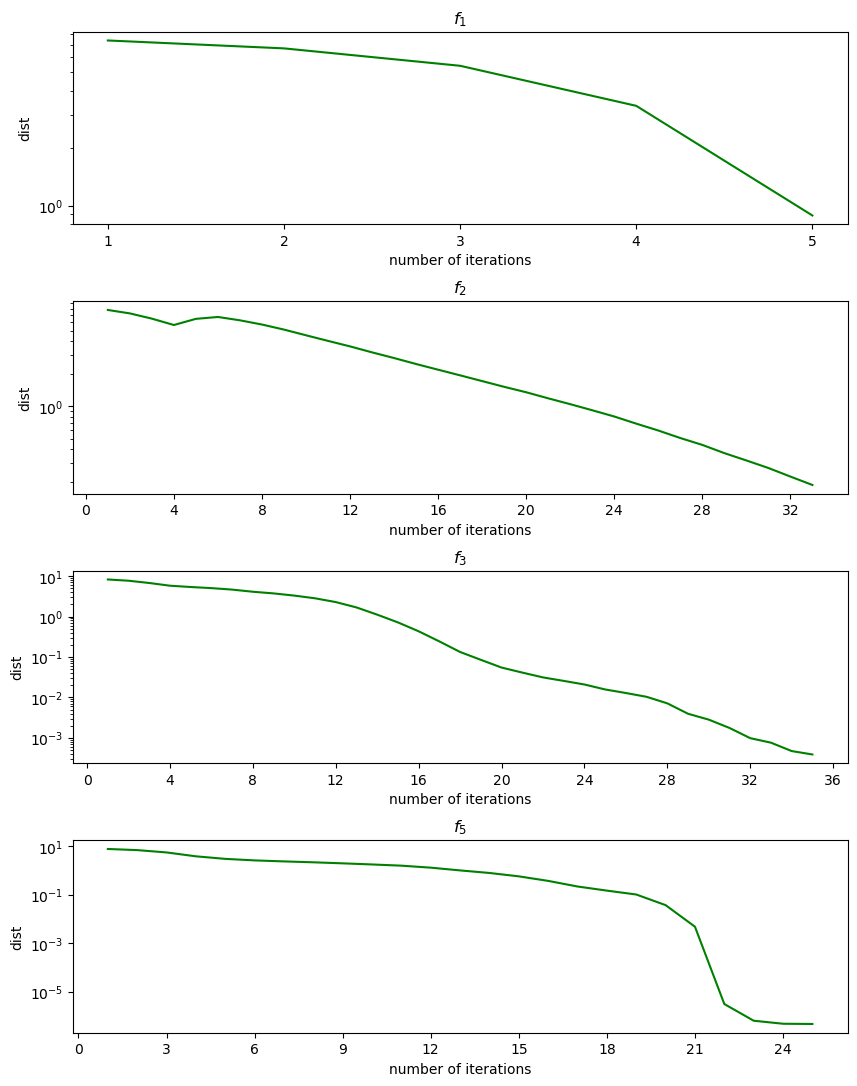
\includegraphics[width=0.7\textwidth]{plt_dist.png}
    \caption{Convergence plot with euclidean distance on the y-axis(log scale)}
  \label{plt1}
\end{figure}

\begin{figure}[]
    \centering
    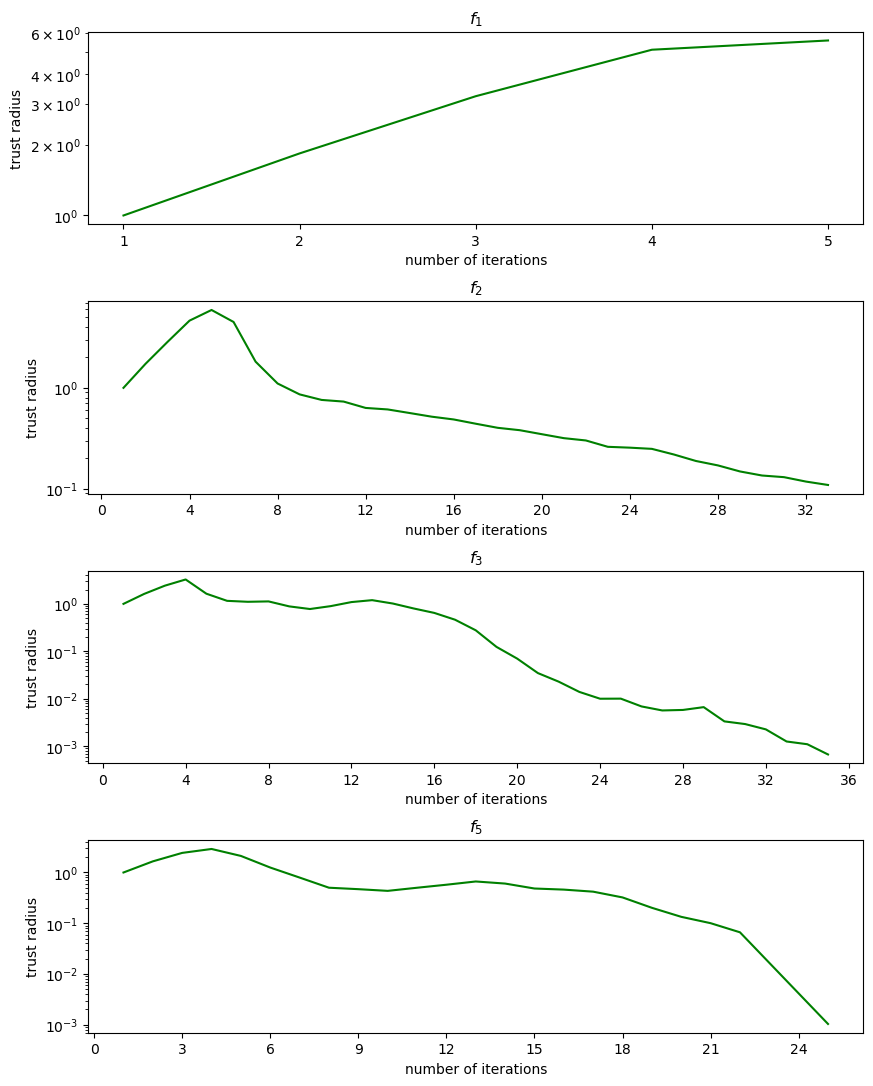
\includegraphics[width=0.7\textwidth]{plt_radius.png}
    \caption{Plot of the trust region radius as a function of number of
      iterations (log scale)}
  \label{plt2}
\end{figure}


\begin{table}[]
\centering
\begin{tabular}{|l|l|l|l|l|l|}
\hline
                 & $f_1$         & $f_2$         & $f_3$       & $f_4$       & $f_5$       \\ \hline
stepest descent & $1.44\cdot10^{-4}$ & $7.59\cdot10^{-4}$ & $1.44\cdot10^{-10}$ & $6.51\cdot10^{-7}$ & $1.13\cdot 10^{-4}$ \\ \hline
newton           & $0.0$      & $8.15\cdot10^{-8}$ & $4.59\cdot10^{-16}$ & $6.4\cdot10^{-7}$  & $4.56\cdot10^{-7}$ \\ \hline
trust region    & $6.11\cdot 10^{-18}$  & $3.17^{-15}$ &  $1.08\cdot10^{-12}$ & n/a & $1.70 \cdot 10^{-7}$ \\ \hline
\end{tabular}
\caption{Average value of distance to the optimum at algorithm termination for 100 random starting points in the interval $[-10,10]$}
\label{table1}
\end{table}

\begin{table}[]
\centering
\begin{tabular}{|l|l|l|l|l|l|}
\hline
                 & $f_1$  & $f_2$  & $f_3$   & $f_4$ & $f_5$  \\ \hline
stepest descent  & $3392$ & $6991$ & $5546$ & $488$ & $52$  \\ \hline
newton           & $1$    & $30$   & $16$   & $29$  & $2 $  \\ \hline
trust region     & $5$    & $32$   & $35$   & n/a   & $24 $ \\ \hline
\end{tabular}
\caption{Average number of iterations until algorithm termination for 100 random starting points in the interval $[-10,10]$}
\label{table2}
\end{table}

\section{Theoretical Part}
In the theoretical part, I choose the second option. \\\\
Problem 4.7 from the Book states:
\[
\min _{p \in \mathrm{R}^{n}} m(p)=f+g^{T} p+\frac{1}{2} p^{T} B p, \quad \text { s.t. }\|p\| \leq \Delta
\]
We assume that $B$ is strictly positive definite. I
will show that the described algorithm converges to $\lambda^*$, s.t
$p(\lambda^*) = p^*$\\\\
We know that $p(\lambda)$ is continuous and
strictly nonincreasing function in the interval $(\lambda_0, \lambda_1)$. (p.85
in the Book). Then, since $\lambda_0 < \lambda' < \lambda_1$,
$\|p(\lambda_0)\| > \Delta$ and $\|p(\lambda_0)\| < \Delta$, it would
hold that $\|p(\lambda_1)\| <  \|p(\lambda')\| < \|p(\lambda_0)\|$. \\\\
Let $\mu(\lambda') = \| p(\lambda') - p(\lambda^{*}) \|$, then we can express
the value of $p$ as a function of $n$, where $n$ is the number of algorithm
iterations:
\[
p_{\lambda'}(n) \leq p(\lambda*) \pm \left(\frac{1}{2}\right)^n\!\mu(\lambda')
\]
Since:
\[
\lim_{n \to \infty} \left(\frac{1}{2}\right)^n = 0
\]
we have that:
\[
\lim_{n \to \infty} p_{\lambda'}(n) = p(\lambda^{*}) = p^{*}
\]
Hence, the algorithm would converge to $p(\lambda^*) = p^*$. Additionally, the
tolerance of this algorithm could be adjusted, since we have an
upper bound on the error. \\\\
For the indefinite case, we can first make the matrix $B$ positive definite, using
one of the methods, suggested in Chapter 3.

\section{Conclusion}
I have implemented the Trust Region algorithm, while solving sub-problem 4.7.
Algorithm manages to find the value of optimum of functions $f_1, f_2, f_3$ and
$f_5$ and its performance is much better than the Seepest Descent method, but
slower than the Newtons method from the last assignment.

\end{document}


%% \section{Convergence Plots}
%% \label{sec:conv}
%% \begin{figure}[H]
%%   \centering
%%   \begin{subfigure}[b]{\textwidth}
%%     \centering
%%     \includegraphics[width=\textwidth]{plt_f_1.png}
%%     \caption{Ellipsoid Function}
%%   \end{subfigure}
%%   \begin{subfigure}[b]{\textwidth}
%%     \centering
%%     \includegraphics[width=\textwidth]{plt_f_2.png}
%%     \caption{Rosenbrock Function}
%%   \end{subfigure}
%%   \caption{Convergence Plots}
%%   \label{plt1}
%% \end{figure}
%% \end{document}
